\documentclass[article,9pt,twocolumn,twoside]{rilabRxiv}
%\documentclass[12pt]{article}
\usepackage[english]{babel}
%\usepackage[letterpaper,top=1in,bottom=1in,left=1in,right=1in,marginparwidth=1.75cm]{geometry}
\usepackage{amsmath}
\usepackage{titlesec}
\usepackage{mathptmx}
\usepackage{graphicx}
\usepackage{longtable}
\usepackage{ltcaption}
\usepackage{tabularx}
\usepackage{adjustbox}
\usepackage{multirow}
%\usepackage[usenames,dvipsnames]{color}
\usepackage{caption}
\usepackage[raggedright]{sidecap} % side captions
\sidecaptionvpos{figure}{t} 
\usepackage[colorlinks=true, allcolors=blue]{hyperref}

%%%%%%%Add comments in color
\newcommand{\jri}[1]{{\small \textcolor{red}{#1}}}
\newcommand{\citex}[1]{{\small \textcolor{red}{CITE(#1)}}}
\newcommand{\X}{{\textcolor{red}{X}}}
\newcommand{\der}{{\textcolor{purple}{X}}}
\newcommand{\so}[1]{{\small \textcolor{blue}{#1}}}
\newcommand{\ashe}{{\textcolor{green}{X}}}
\newcolumntype{b}{X}
\newcolumntype{s}{>{\hsize=.5\hsize}X}

% Set supplement numbers to S and start counting newly
\newcommand{\beginsupplement}{%
        \setcounter{table}{0}
        \renewcommand{\thetable}{S\arabic{table}}%
        \setcounter{figure}{0}
        \renewcommand{\thefigure}{S\arabic{figure}}%
     }


\title{The Impact of Selection on the Efficacy of Integrative eQTL and QTL Analysis in a Multi-Parent Population}

\author[$\ast$,1,2]{Nicholson, Sarah G.O.}
\author[1]{Crow,Taylor}
\author[1]{Perkins,Taylor}
%\author[2,3]{Hudson, Asher I.}
\author[3]{Praud, S\'ebastien}
\author[3]{Dubreuil, Pierre}
\author[3]{Tixier, Marie-Helene}
\author[2,4,5]{Ross-Ibarra, Jeffrey}
\author[1]{Runcie, Daniel E.}

\affil[1]{Dept. of Plant Sciences, University of California, Davis, CA, USA}
\affil[2]{Dept. of Evolution and Ecology, University of California, Davis, CA, USA}
\affil[3]{Limagrain, Chappes, France}
\affil[4]{Center for Population Biology, University of California, Davis, CA, USA}
\affil[5]{Genome Center, University of California, Davis, CA, USA}
\affil[$\ast$]{Dept. of Plant Sciences and Department of Evolution and Ecology, University of California, Davis, CA, USA}
%\affil[$\ddagger$]{Genome Center, University of California, Davis, CA, USA}


%\keywords{Keyword one, keyword 2}

\runningtitle{Running title} % For use in the footer
\runningauthor{Nicholson \textit{et al.}}


%%% Abstract %%%%%%%%%%%%%%%%%%
\begin{abstract}
Gene expression is a crucial intermediary between genetic variation and phenotype.
Therefore, many studies have sought to incorporate gene expression in QTL mapping and GWAS to determine the underlying mechanisms of QTL for complex traits.
However, the success of these integrative eQTL-QTL studies in identifying candidate genes and explaining genetic variation in complex traits has been mixed.
Here, we use gene expression data from a population of MAGIC F1s derived from 16 diverse inbred maize lines to identify associations between genetic, transcriptomic, and phenotypic variation and highlight the impact of selection on the genetic architecture of gene expression traits.
Leveraging the multi-allelic nature of a MAGIC population, we test for correlation between effect sizes of overlapping local-eQTL and QTL to assess co-localization and identify 5 potential candidate genes for two flowering time QTL.
In addition, we show evidence of both historical and recent stabilizing selection acting on gene expression traits and find a significant relationship between the correlation of local-eQTL and complex traits and the magnitude of local-eQTL effect sizes.
Both these findings provide support for the strong impact of stabilizing selection on gene expression, particularly for genes associated with complex traits.
\end{abstract}
%%%%%%%%%%%%%%%%%%%%%%%%%%

\setboolean{displaycopyright}{true}

\begin{document}

\maketitle
\thispagestyle{firststyle}
\correspondingauthoraffiliation{
Dept. of Plant Sciences, University of California, Davis, CA, USA
E-mail: sgodell@ucdavis.edu}
\vspace{-11pt}%

\section{Introduction}
\lettrine[lines=2]{\color{color2}G}{} ene expression acts as a major intermediary between genotype and phenotype.
There have, therefore, been many attempts to explain the association between genetic variants and complex traits by linking those variants to variation in the expression of some candidate gene.
Expression QTL (eQTL) are regions of the genome where genetic variation is associated with variation in gene expression.
Integrative approaches combining eQTL and GWAS or QTL mapping have been used in multiple species for the purposes of plant and animal breeding and of furthering our understanding of the underlying biological mechanisms of complex traits.
Many studies have used an integrative systems biology approach to identify genes and genetic variants that are associated with quantitative traits in a variety of organisms including \emph{Drosophila} \citep{Ayroles,PassadorGurgel,Harbison}, humans \citep{Naukkarinen}, mice \citep{Lan}, chickens \citep{Roux}, pigs \citep{Liu4}, \textit{Brassica napus L.}\cite{Yu3}, and maize \citep{Baute,Pang,Miculan}, among others.
\par
There is good reason to suspect that many variants associated with complex traits will also have an eQTL that mediates that trait.
A large amount of GWAS hits are found in non-coding regions, suggesting that they contribute to complex traits through modulation of gene expression \citep{Maurano,Gusev}.
These variants also tend to be in accessible chromatin regions in relevant cell types, potentially only impacting the associated trait in specific tissues or developmental stages \citep{Trynka}.
GWAS hits are likely to be associated with expression of neighboring genes and are enriched within eQTL in relevant tissues \citep{Trynka2, Nicolae}.
A number of studies have applied such techniques to successfully identify candidate genes whose expression helps explain variation in complex traits \citep{Liu4,Miculan,Pang,Roux,Yu3}.
In maize, there are numerous examples of local- or \textit{cis}-eQTL underlying complex traits such as flowering time and circadian rhythm (ZCN8 \citep{Guo} and ZmCCT9 \citep{Huang3}), both traits that were crucial to the adaptation of maize to more temperate climates during domestication \citep{Navarro,Bouchet,Hung,Yang}.
\par
However, a large proportion of GWAS hits are not explained by identified eQTL \citep{Chun,Umans,Connally}.
Only about 25\% of loci were found to be shared among GWAS hits for auto-immune diseases and eQTL found in relevant human immune-cell populations \citep{Chun}.
In a comparison of \textit{cis}-eQTL in humans, just 11\% of the heritability of complex traits were mediated by gene expression \citep{Yao}.
There have been multiple proposed explanations for this lack of overlap.
Some of the disparity may be due to genetic variants impacting other molecular mechanisms, such as alternative splicing, although splicing QTL were found to explain only a small proportion of variation in complex traits \citep{Mu}.
Similarly, "phenotypic buffering", where eQTL correlated poorly with protein and  metabolite levels, was observed in \textit{Arabidopsis} \citep{Fu}.
The impact of eQTL on complex traits may be mitigated by downstream effects, such that the variance explained is small, despite the eQTL playing a role in mediating the trait. 
The justification for this phenomenon is that  biological networks must be robust to perturbation, and so genetic variants with potentially large effects on traits impacting organismal fitness may be attenuated by the biological network \citep{Hu2}.
Another explanation is that many eQTL only affect complex traits in very specific contexts; while cell-type-specific eQTL added a small amount of variation explained, there is some evidence that eQTL at certain developmental stages, or in response to outside stimulus may play a larger role in explaining GWAS loci \citep{Mu,Snoek}.
\par
% Low power and Mostafavi
Yet another potential explanation is that the power of eQTL studies is not sufficient to capture smaller effect eQTL that mediate complex traits.
However, as the size of eQTL studies has grown, although the amount that eQTL can explain GWAS loci for complex traits has increased, it has only increased moderately with sample size \citep{Umans}.
Part of this may be due to the fact that natural selection impacts the power of GWAS and eQTL studies differently \citep{Mostafavi}.
eQTL studies may be inherently under-powered to detect trait-associated eQTL, as large effect eQTL that are associated with a complex trait are more likely to be brought to lower frequency in the population by negative selection.
GWAS hits tend to be in regions under stronger selective constraint, where we are under-powered to detect eQTL.

\begin{figure*}[ht!]
\centering
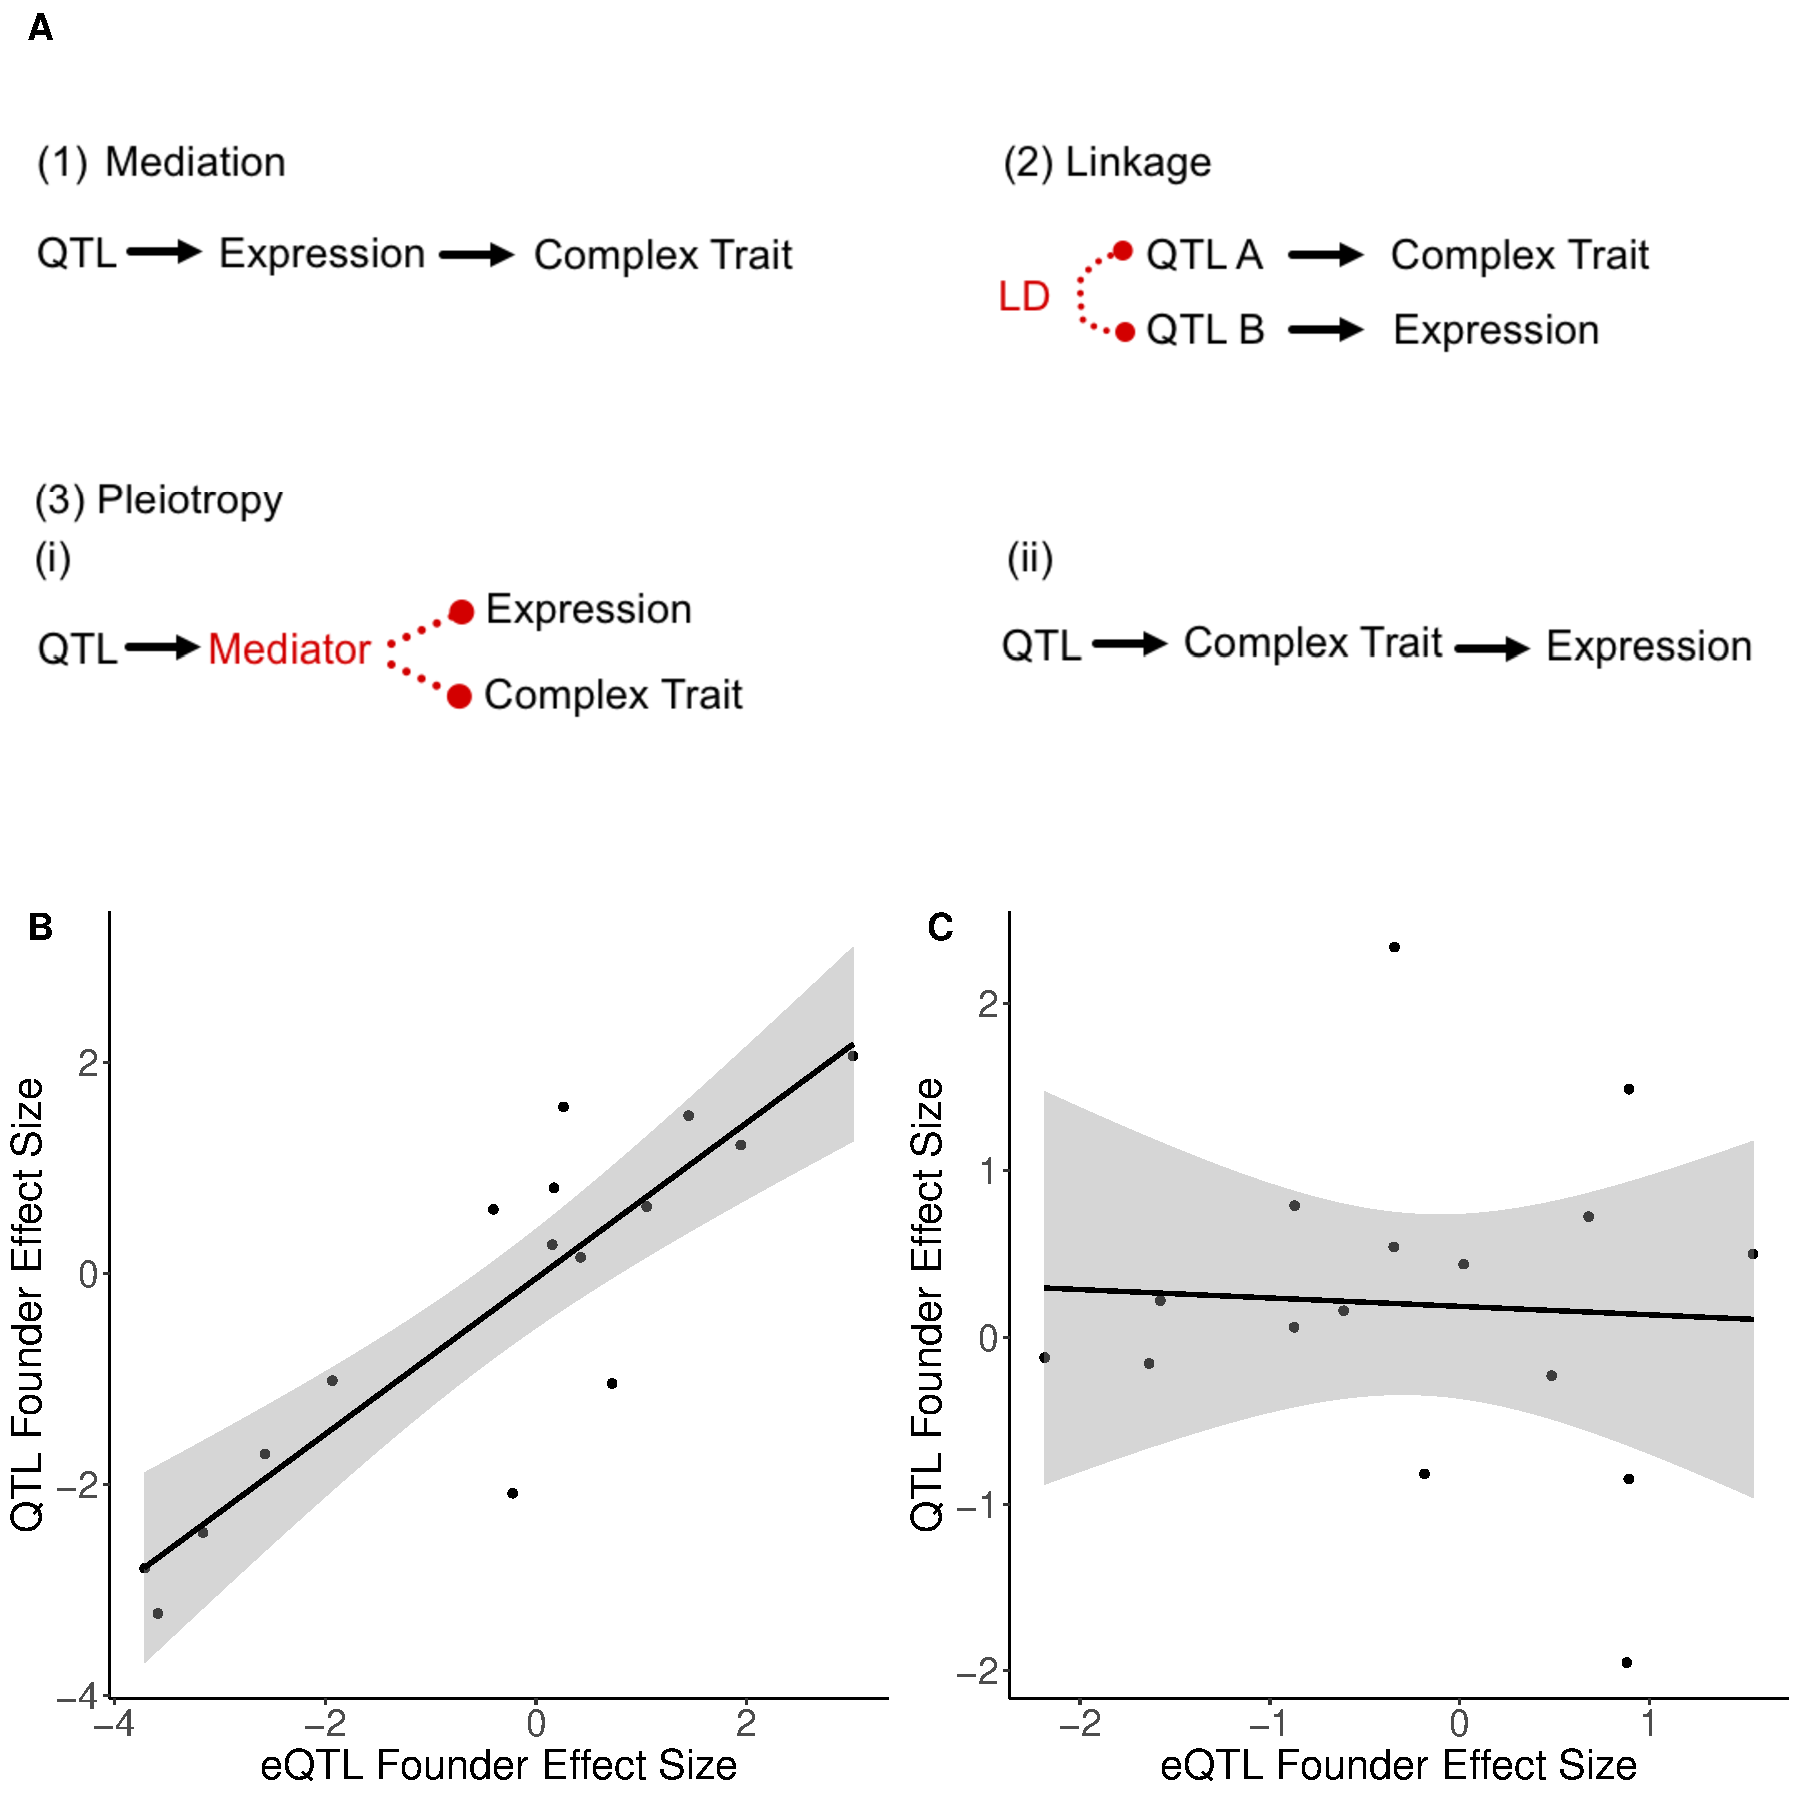
\includegraphics[width=0.7\textwidth,height=4in]{figures/scenarios_figure.pdf}
\caption{\textbf{Relationships Between Gene Expression and Complex Traits} 
\textbf{(A)}. Different scenarios of relationships between genetic variation, gene expression, and complex traits.
\textbf{(B)}. An example of a significant correlation between QTL effect sizes for complex traits and eQTL effect sizes for expression of a gene. 
 We expect this pattern to be observed in the cases of mediation (A1) and pleiotropy (A3i \& A3ii).
 \textbf{(C)}. An example of unrelated QTL and eQTL effect sizes. We expect this pattern to be observed in the cases of linkage (A2)}
\label{fig:scenarios}
\end{figure*}

Evolutionary theory holds that large effect variants tend to be deleterious.
We see evidence of stabilizing selection in most complex traits, with extreme phenotypes being selected against.
For molecular traits such as gene expression, it has also been shown that alleles associated with extreme phenotypes are similarly harmful \citep{Zhao,Kremling2}.
Stabilizing selection brings alleles with large effects to lower frequency in populations, and, therefore, large effect alleles tend to be rare.
Previous studies in humans and maize have shown an enrichment of rare alleles upstream of genes with extreme (either very high or very low) expression relative to the population, a pattern which has been termed dysregulation \citep{Zhao,Kremling2}.
Further, \cite{Kremling2} found that the degree of dysregulation of an individual was predictive of a reduction in seed weight, used as a proxy for fitness, in a maize association panel.
All this together paints a picture of stabilizing selection acting not just on complex traits, but on gene expression traits as well, maintaining intermediate phenotypes in a population.
Our population presents a unique opportunity to expand upon this picture by looking at both historical and recent selection and its impact on gene expression as an intermediate of complex traits.
\par
One hurdle in linking eQTL to QTL for complex traits is that, even if there is physical overlap observed, it is not guaranteed that an eQTL is mediating the effect of the overlapping QTL.
This overlap could instead be due to linkage or pleiotropy (\hyperref[fig:scenarios]{Figure 1A})\citep{Yao}.
In the case of linkage, the QTL and eQTL variant are different linked loci, but for mediation and pleiotropy, the same locus is associated with both the eQTL transcript and complex trait.
Multiple methods have been developed to attempt to disentangle these three scenarios \citep{Porcu,Zhu}.
Co-localization tests have been developed to determine if the eQTL and GWAS hit are actually caused by the same underlying genetic variant, ruling out linkage \citep{Hormozdiari}.
Transcriptome-wide association studies (TWAS) combine summary statistics from GWAS and eQTL mapping to detect association with imputed gene expression values \citep{LiRitchie}.
TWAS has been applied in multiple instances used to supplement GWAS in humans \citep{Gusev2} and maize \citep{Kremling}, as well as many other organisms.
Although powerful, one downside of TWAS is that it cannot rule out that the association between gene expression and the complex traits is due to either pleiotropy or linkage \citep{Yao}.
\par
Multi-parent Advanced Generation Intercross (MAGIC) populations have been used in integrative eQTL-QTL studies in a number of species in the hopes of understanding the biological mechanisms underlying QTL \citep{DellAcqua,Miculan,Snoek}.
Unlike association panels, mapping populations lack population structure, as all individuals are approximately equally related to one another.
In addition, the breeding scheme of the population should theoretically bring all founder alleles to appreciable and approximately equal frequency, improving our ability to estimate founder effect sizes.
In association panels, estimates of the effect sizes of rare allele are more imprecise.
Compared to bi-parental mapping populations, MAGIC populations possess more genetic diversity.
Finally, in terms of measuring gene expression, MAGIC populations provide an advantage in that they can measure the expression of parental gene copies in diverse genetic backgrounds.
\par
This population allows for the use of a parental multi-allelic model, instead of a bi-allelic model \citep{Odell}.
This means that we are able to look for association of eQTL and QTL by calculating the correlation of founder effect sizes.
This method rules out linkage as a reason for overlap between eQTL and QTL, identifying candidate genes that potentially mediate complex traits, although it cannot differentiate mediation from pleiotropy (\hyperref[fig:scenarios]{Figure 1A}).
Pleiotropy has a large number of definitions and classifications \citep{Paaby,Solovieff,Hu2}.
For the scope of this paper we will group them into two scenarios: (i) the variant correlates with the expression of the eQTL transcript and the complex trait through some mediator trait, or (ii) the variant impacts the complex trait, which then mediates expression of the eQTL transcript (\hyperref[fig:scenarios]{Figure 1A}, 3i \& 3ii).
As an example of scenario (i), a marker might be correlated with flowering because it is associated with senescence and also correlated with a gene that is more highly expressed during senescence.
Earlier flowering individuals will undergo senescence earlier, so the expression of genes involved in senescence will be correlated with flowering time, although they do not mediate flowering.
For scenario (ii), we might have a QTL associated with flowering, which might, therefore, be correlated with expression of a gene that is highly expressed during flowering, but does not induce flowering. 
In these scenarios, the genetic effects of founder alleles on both complex trait and gene expression may be correlated without gene expression mediating the trait itself.
\par
Maize (\textit{Zea mays ssp. mays}) is an important model organism with vast genetic and phenotypic resources as well as being an agronomic staple crop.
Forward genetics have been used in maize to identify the genetic basis of several agronomically-important complex traits using both QTL mapping and GWAS \citep{Buckler,Li4,Wallace,Xue}.
Likewise, multiple studies have sought to identify eQTL in maize \citep{Liu6,Pang,Wang3}.
\par
In this study, we applied a systems genetics approach using genotype, phenotype, and expression data all from the same population of MAGIC F1 lines.
The use of a founder multi-allelic model allowed us to assess the association of eQTL and QTL effect sizes as a means of identifying genes related to complex traits.
Systems genetics approaches to understanding complex traits also incorporate information on biological networks \citep{CivelekLusis}.
This study is distinct in performing both QTL mapping and eQTL mapping in a single population, pairing expression data with phenotype data both from the same field and from a number of different environments.
An advantage of this design is that the eQTL and QTL studies are performed on the same population, making them more similarly powered than many integrative eQTL-GWAS studies due to approximately equal sample sizes.
The gene expression data, although only taken from one tissue type, mature leaf tissue, is from multiple relevant timepoints for the complex traits being studied.
We sought to answer the following questions:
(1) What eQTL are present in this population?, 
(2) How well can correlations of founder effect sizes between eQTL and QTL identify candidate genes?, and
(3) What are the effects of selection on gene expression traits?
\section{Materials and Methods}
\label{sec:materials:methods}
\subsection{MAGIC Population}
The BALANCE MAGIC population was generated using 16 diverse inbred maize lines (Table \ref{tab:founder_suptable}). 
The lines were crossed in a funnel crossing scheme \citep{Odell}. 
After multiple generations of outcrossing, double haploids of the synthetic lines were created to make the lines entirely homozygous. 
These double haploids were then crossed to an inbred tester, MBS847, to form MAGIC F1s.
\subsection{Sample tissue collection}
Between 290 and 340 of the MAGIC F1 genotypes were grown up in two fields in St. Paul, France in 2017, with two plots of 80 plants planted per genotype.
One field was given a standard watering regime, while the other was given a water-deficit treatment, where water was withheld from July 9 to July 29, 2017, overlapping with the onset of flowering, after which normal watering was resumed. 
Mature leaf tissue from leaves at about the V13 stage of each genotype were collected at multiple time points over the course of about two weeks.
Two well-watered time points were collected at the start and end of the drought treatment, and five water-deficit time points were collected spread out every few days over the course of the drought treatment.
For each genotype, hole punches of leaf tissue from five plants were pooled in a tube and snap-frozen in liquid nitrogen.
Tissue was sampled by in the morning by four groups, with all samples taken within an hour of each other.
The order of movement for groups sampling through the field was alternated per timepoint. 
Phenotype data was also measured in the water-deficit field where tissue was collected, which we refer to as St.Paul, 2017 \#1.
\subsection{Library preparation, quality control and analysis}
The leaf tissue samples were prepared into libraries using the BrAD-Seq protocol \citep{Townsley}. 
The RNA-Seq libraries were sequenced by IDSeq using Illumina 150bp paired-end short read sequencing.
Samples with extremely high adapter content or fewer than 1 million uniquely mapped reads were removed. 
We used trimmomatic, fastqc, and multiqc \citep{Bolger,Andrews,Ewels} to trim adapter sequences and assess library quality.
After quality filtering, we were left with 4 water-deficit timepoints with enough high-quality samples to perform expression-QTL mapping (T12, T18, T20, and T27).
The timepoint numbers reference the date the timepoint was taken.
Reads were aligned using 2-pass alignment with the software STAR \citep{Dobin}.
We estimated read counts per gene with STAR using the B73 v4 reference genome and annotation \citep{Jiao} .
Gene counts from STAR were normalized using limma voom into log2 counts per million (log2cpm), filtering out genes that had fewer than 15 individuals with at least 5 log2cpm expression \citep{Law}.
\subsection{local-eQTL Identification}
In order to identify local-eQTL, we used the software GridLMM \citep{Runcie1} to identify local-eQTL within recombination blocks.
We did this using founder probabilities estimated from the population genotype data \citep{Odell}.
Founders with low representation were dropped from a test to improve estimation of effect sizes.
A founder was dropped from a test for a marker if there were fewer than 4 individuals with a probability for that founder greater than 0.75 at that marker.
The first three PCs of the normalized gene count data were used as covariates in order to account for variation due to sampling time and batch effects.
For each gene, we tested for association between its variation in expression between genotypes and founder identity in the recombination block the gene was located in.
We weighted each gene using the weights calculated by voom using the weights argument in the GridLMM\_ML function.
The significance of local-eQTL were determined using a 10\% FDR threshold using the qvalue package \citep{Storey}.
The model fit for each gene-marker pairing is shown here:
    \begin{equation}
    \label{eqn:gridlmm2}
    y_g = \mu + PC_{1-3} + X_{Fi}{\beta_{Fig}} + Zu + \epsilon
    \end{equation}
    where $y_g$ is the response variable for gene $g$, $\mu$ is the population mean, $PC_{1-3}$ is a matrix of eigenvectors from the top three principal components, $X_{Fi}$ is a $n \times f-1$ matrix for marker $i$ and $x_{fni}$ is the probability that at site $i$, individual $n$ was derived from founder $f$ and $\beta_{Fig}$ is the effect size of each founder allele on expression of gene $g$, $Z$ is the design matrix, $u \sim \mbox{N}(0,\sigma^2_u \bf{K})$ is the random effects of markers across the rest of the genome using the genomic relationship matrix, $K$, and $\epsilon$ is the error.
The genomic relationship matrix, $K$ was generated from the 600K SNP data using a leave-one-chromosome-out (LOCO) method.
\subsection{Whole-genome distal-eQTL scan}
We wished to test for distal-eQTL for individual genes that might be identified across the whole genome.
A model similar to Equation \ref{eqn:gridlmm2} was used, using the first three PCs of normalized gene expression as covariates.
Founders with low representation were dropped from a test to improve estimation of effect sizes in the same way described for local-eQTL.
In order to exclude markers that were in LD with the local marker, we calculated the additive genetic effect on expression of a gene ($\alpha_{ig}$) for all markers, and dropped markers from the analysis if the correlation between the local genetic effect and the distal genetic effect was $\ge$ 0.2.
Additive genetic effects for a marker were calculated as
    \begin{equation}
    \label{eqn:bvs}
    \alpha_{ig} = X_{Fi}{\beta_{Fig}}
    \end{equation}
    where $\alpha_{ig}$ is the additive genetic effect of marker $i$ on expression of gene $g$.
The effect sizes ($\beta_{Fig}$) were obtained from the output of Equation \ref{eqn:gridlmm2}.
We weighted each gene using the weights calculated by voom using the weights argument in the GridLMM\_ML function.
To account for multiple testing, we used a 10\% FDR significance threshold accounting for the number of markers and number of genes being tested.

\subsection{Identification of QTL Candidate Genes}
We wished to determine if any local-eQTL overlapping with QTL support intervals (SIs) represented reasonable candidate genes for the QTL.
To do this, we calculated the Pearson's correlation coefficient ($r$) between founder effect sizes for local-eQTL and the overlapping QTL (\hyperref[fig:scenarios]{Figure 1}).
Local-eQTL were said to be overlapping a QTL if the eQTL variant was within the QTL support intervals.
We used QTL and QTL SIs found by \cite{Odell} at a 10\% significance threshold using a founder multi-allelic model ($QTL_F$).
A total of 54 QTL were used from 7 different environment-years and 7 phenotypes.
In order to assess if correlations were larger than expected by chance, we performed the same correlation of effect sizes for distal-eQTL whose variants overlapped with the same QTL.
For all correlations, we used Fisher's Z transformation to normalize $r$ values and get consistent measures of difference in correlations ($|z|$).
For each QTL, we measured the difference between the most correlated local eQTL's $z$ value ($\max {|z_{local}|}$) and the most correlated distal eQTL's $z$ value ($\max {|z_{distal}|}$) as:
    \begin{equation}
    \label{eqn:zdiff}
    \delta_{z} = \max_{|z_{local}|} - \max_{|z_{distal}|}
    \end{equation}
If $\delta_{z} < 0$, it suggests that $\max_{|z_{local}|}$ is small, not because there is a lack of power to detect high correlations, but that local-eQTL do not explain the effect of the QTL (because expression was not measured in the appropriate context, the QTL is affected by expression in trans, etc.).
However, if $\delta_{z} > 0$, the gene with the $\max_{|z_{local}|}$ eQTL is a potential candidate gene for the QTL.
To correct for the size of the support interval and multiple testing, for each QTL, we performed 100 random permutations where in each permutation, we collected a random sample of distal-eQTL and local-eQTL matching the true number of overlapping eQTL for a QTL.
From these random samples, we calculated the highest $|r|$ for the local-eQTL and the distal-eQTL groups.
We were then able to make a null distribution of $\delta_{z}$ values for each QTL to assess if the true $\delta_{z}$ was larger than expected by chance using 5\% significance threshold.

\subsection{Imputation of MAGIC lines}
The 16 founders and the tester were sequenced with Illumina whole-genome sequencing.
We called SNPs by aligning to the B73 v4 reference genome using GATK best-practices \citep{VanDerAuwera}.
Using founder probabilities obtained from the 600K genotype data using R/qtl2, we imputed the founder WGS genotypes for 325 MAGIC lines \citep{Broman}.
For each SNP, we obtained the probability that a line possessed the alternate allele ($a_{nj}$) as
    \begin{equation}
    \label{eqn:allele_prob}
      a_{nj} = \Sigma_{f=1}^F x_{fni}b_{fj}
    \end{equation}
where $x_{fni}$ is the probability that at site $i$, individual $n$ was derived from founder $f$, $b_{fj}$ is either 0 or 1, depending on whether founder $f$ has the alternate allele at SNP $j$, with $j$ located within recombination block $i$.

\subsection{Identification of Rare Alleles}
We identified rare alleles (0.01 $\le$ MAF $\le$ 0.05) in the maize HapMap3 that were also present in the 16 founders and tester of the BALANCE population \citep{Bukowski}.
We filtered out variants that were not bi-allelic.
In addition, we filtered out variants where B73 possessed the minor allele, to avoid bias from B73 being a founder in the population.
In total, there were 2,075,860 rare variants present in both HapMap3 and our population.
Of these, 150,280 variants were present in the tester line, MBS847.

\subsection{Founder Allele Frequencies for Genes Associated with Complex Traits}
We grouped local-eQTL by whether they overlapped with a QTL SI and had $|r| \ge 0.3$ for founder effect size correlations with that QTL.
For local-eQTL that overlapped with QTL for multiple complex traits, we grouped the local-eQTL with the trait that had a higher $|r|$.
We then fit two linear models of founder allele frequencies by Z-score bin and absolute Z-score bin, respectively.
For the model with Z-scores, we performed a Tukey test to see if the estimate of the second degree polynomial was significantly different among local-eQTL associated with complex traits and local-eQTL that were not associated with any of the measured complex traits.
For the model with absolute Z-scores, we performed a Tukey test to see if the slopes and intercepts of the regression lines were significantly different among local-eQTL associated with complex traits and local-eQTL that were not associated with any of the measured complex traits. 

\begin{table*}[!t]
    \centering
    \caption{\textbf{eQTL Identified Across Timepoints} \label{tab:eqtltable}}
    \begin{adjustbox}{max width=0.9\textwidth,center}
    \begin{tabular}{c c c c c c}
    \hline \\
    Timepoint & n & local-eQTL & distal-eQTL & \# distal-eQTL genes & Total \# Genes \\
    \hline \\
     T12 & 83 & 14,510 & 27,804 & 11,612 & 16,218\\
     T18 & 143 & 16,901 & 30,760 & 13,730 & 17,516\\
     T20 & 220 & 17,630 & 31,777 & 14,019 & 18,062\\
     T27 & 194 & 17,372 & 30,656 & 13,540 & 17,823\\
     Total & -- & 66,413 & 120,997 & 18,591 & 18,950 \\
     \hline
    \end{tabular}
    \end{adjustbox}
    %\\\hline
\end{table*}


\subsection{Data availability}
Supplemental files and figures will be made available through FigShare (https://figshare.com/s/d37551d5932a8d401f03).
Code used to run analyses can be found at \url{https://github.com/sarahodell/bg_rnaseq}.

%%%%%%%%%%%%%%%%%%%%%%%%%%%%%%%%%%%%%%%%%%%%%%%%%%%%%%
\section{Results}
%%%%%%%%%%%%%%%%%%%%%%%%%%%%%%%%%%%%%%%%%%%%%%%%%%%%%%

\begin{figure*}[ht!]
\centering
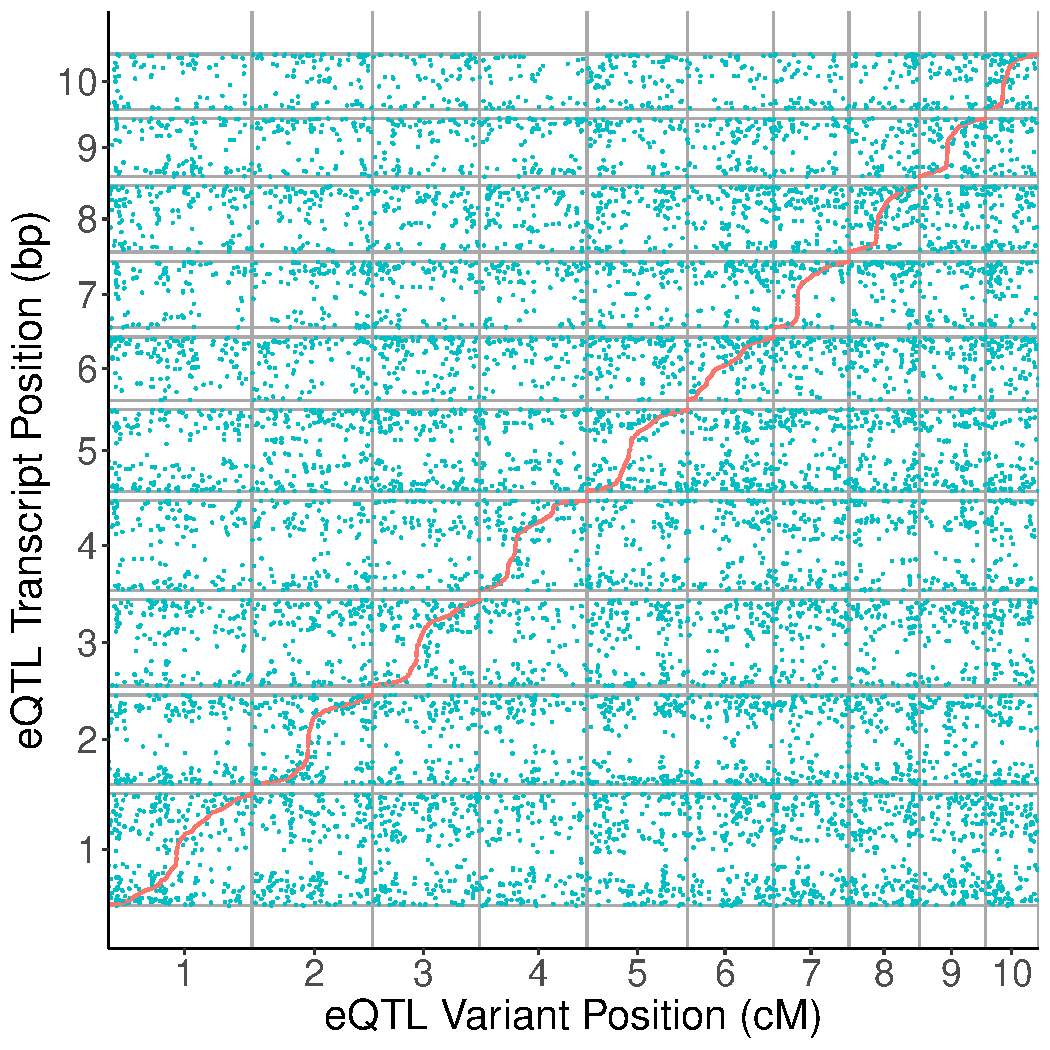
\includegraphics[width=0.9\textwidth,height=6in]{figures/WD_0712_top5k_cis_trans.pdf}
\caption{\textbf{local- and distal-eQTL identified in T12.} eQTL identifed in timepoint T12 for the top 5,000 most highly expressed genes. The position of the eQTL variant in genetic distance is shown on the x-axis and the physical position of the eQTL transcript is shown on the y-axis as the mid-gene location. The color of each point represents whether it was found as a local- (red) or distal-eQTL (blue). The grid lines delineate the 10 chromosomes, with dark grey lines demarcating the start and ends of chromosomes.}
\label{fig:cistransfigure}
\end{figure*}

\subsection{Single-gene eQTL identification}
%local eQTL
We measured gene expression from leaf tissue of MAGIC hybrid lines in four timepoints over the course of flowering.
In the four timepoints, the first three principal components accounted for 17.1 \%, 18.1\%, 14.3\%, and  24\% of variation, respectively.
In the first timepoint, T12, the first PC was highly correlated with the plates of the samples ($r=0.82$), but there was less of a correlation between plate and PCs for the three other timepoints (Figures \ref{fig:chapter2_t12pc}-\ref{fig:chapter2_t27pc}).
The sampling group and order of sampling seemed to be captured well by the second PC in all four timepoints (Figures \ref{fig:chapter2_t12pc2}-\ref{fig:chapter2_t27pc2}).

We wished to identify local-eQTL in the population, which we considered to be variants that were associated with the expression of genes in the same recombination window as the variant.
To account for variation due to plate and sampling order, the first three PCs were used as covariates.
We identified a total of 66,413 local-eQTL associated with 18,769 genes (Figure \hyperref[fig:cistransfigure]{Figure 2.2}, \hyperref[tab:eqtltable]{Table 1}).
The majority of local-eQTL were found in multiple timepoints (median = 4, mean = 3.54), with 13,268 genes possessing local eQTL in all four timepoints and 1,009 genes only having local-eQTL at one timepoint.
Most genes were found to have an eQTL in the local recombination window, with 89\% of genes tested having local-eQTL in T12, 96\% in T18, and 97\% in both T20 and T27.
The true negative ($\pi_0$) value was estimated to be 0.13.
The amount of variation in gene expression explained by local-eQTL ranged from $<$1\% to 97\% (median=14\%, mean=18\%).
\par
We performed a whole-genome scan to test for the presence of distal-eQTL.
Here, we defined distal-eQTL as genetic variants associated with variation in gene expression of a gene located outside of the recombination window of the variant ($|r(\alpha)| \le 0.2$, see Equation \ref{eqn:bvs}).
In total we found 120,997 significant distal-eQTL at a 10\% FDR associated with 18,591 different genes (\hyperref[tab:eqtltable]{Table 1}).
The true negative rate ($\pi_0$) for distal-eQTL was estimated to be 0.69.
Of these distal-eQTL, 95,176 (79\%) of these associations were between a gene and variant on different chromosomes.
The number of distal-eQTL found in each timepoint seemed to be associated with the sample size of the timepoint.
Most genes (89\%) had distal-eQTL in more than one timepoint, with distal-eQTL found for 2,049 genes in one timepoint, 4,270 genes in 2 timepoints, 6,776 genes in 3 timepoints, and 5,496 genes in all four timepoints.
Very few distal-eQTL were consistent across timepoints.
The most significant  marker of a distal-eQTL was shared across timepoints for only 1,474 distal-eQTL (1.2\%).
This is consistent with findings that distal- and \textit{trans}-eQTL tend to be context specific \citep{Snoek,Mu,Vosa,vanNas}.

\begin{figure*}[!ht]
%\begin{SCfigure*}
\centering
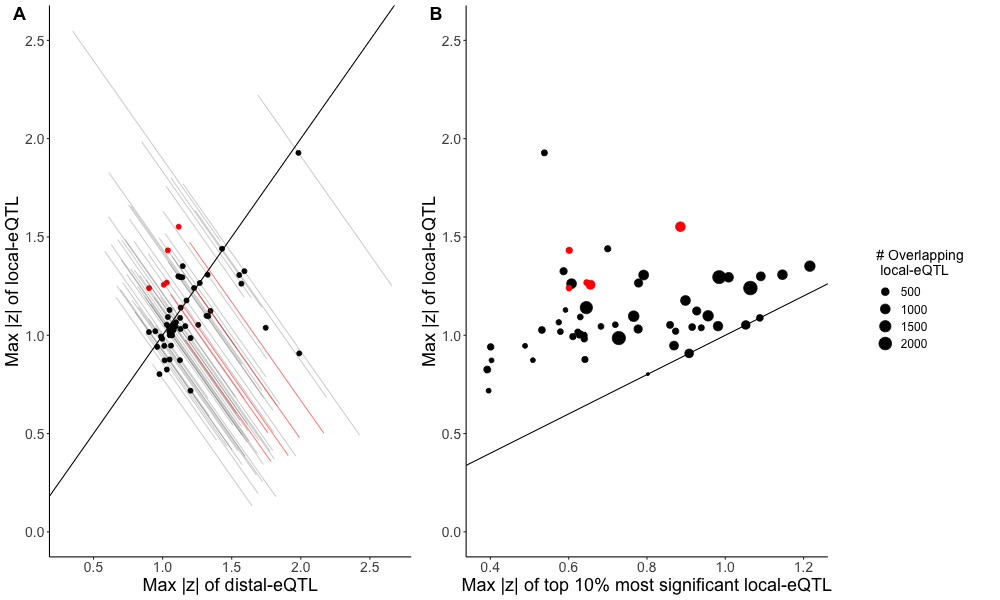
\includegraphics[width=0.9\textwidth,height=3.5in]{figures/chapter2_figure3_v2.png}
%\captionsetup{width=.9\columnwidth}
%\protect\rule{0ex}{4ex}
\caption{\textbf{eQTL Associated With Complex Traits Tend to have Small Effect Sizes}
Red points are QTL with candidate genes, whose $\delta_{z}$ was greater than 95\% of random permutations. \textbf{A} Each point represents a QTL. The x-axis shows the maximum absolute Z-transformed Pearson correlation coefficient ($|z|$) of any distal-eQTL overlapping the QTL support interval (SI). The y-axis shows $|z|$ of any local-eQTL overlapping the QTL SI. The points above the diagonal represent QTL whose $\max {|z_{local}|}$ is greater than the $\max {|z_{distal}|}$. Thin diagonal lines represent the 95\% permutation null distribution for that QTL (see Methods). \textbf{B}. The x-axis shows the $\max {|z_{local}|}$ for the top 10\% most significant eQTL overlapping the QTL support interval. The y-axis shows the $\max {|z_{local}|}$ for all eQTL within the SI. The size of the points shows the number of eQTL overlapping the QTL SI. Points above the diagonal are QTL whose $\max {|r_{local}|}$ eQTL was not in the top 10\% most significant eQTL in the SI.}
\label{fig:candidates}
\end{figure*}

\subsection{distal-eQTL Hotspots}
There were 17,036 distal-eQTL peaks that were significantly associated with more than one gene.
For these distal-eQTL hotspots, the average number of genes associated with a locus was 7 ($\sigma$ = 4.8, median = 6, Figure \ref{fig:chapter2_supfigure1}).
The largest distal-eQTL hotspot was in T27, where a 126 kb window on chromosome 8 was associated with 62 genes.
This region overlaps with the large flowering time QTL \textit{qDTA8}/\textit{qDTS8}.
There were 3 local-eQTL in the window for Zm00001d010974, Zm00001d010975, and Zm00001d010976.
One of these genes, Zm00001d010975, loaded on a factor, TGE T27-F4, with 42 of the 62 distal-eQTL genes.
Zm00001d010975 encodes IQ-domain 21, a calmodulin binding protein, and overlaps with a GWAS hit for flowering time \citep{vanInghelandt}.
This region was also a distal-eQTL hotspot in the other timepoints, although there were fewer genes with distal-eQTL in these timpoints (21 in T12, 7 in T18, and 12 in T20).
Only one gene, Zm00001d011457 , had a distal-eQTL in this region in more than one timpeoint (T12 and T20).
\subsection{QTL Candidate Genes}
By estimating effect sizes of founder alleles, we gain the ability to assess correlation of effect sizes between gene expression and complex traits.
Genes with local-eQTL that both overlapped QTL support intervals (SIs) and whose local-eQTL founder effect sizes correlated strongly with those of the overlapping QTL are reasonable candidate genes for involvement in the complex trait for that QTL.
We determined candidate genes by looking at local-eQTL with variants that overlapped with QTL support intervals (SI).
The distribution of correlations for local- and distal-eQTL varied by phenotype and by specific QTL (Supplemental Files \href{run:./figures/local_distal_r_density.pdf}{7} \& \href{run:./figures/local_distal_r_hist.pdf}{8}).
A gene was considered to be a candidate gene if its local-eQTL had the highest correlated effect size ($|r|$) to the overlapping QTL, with that correlation being significantly larger than that of overlapping distal-eQTL (\hyperref[fig:candidates]{Figure 3}A, see \hyperref[sec:materials:methods]{Methods}).
Of the 54 QTL found in this population across 7 environments, only 5 QTL possessed strong candidate genes that passed our selection criteria (\hyperref[fig:candidates]{Figure 3}A, \hyperref[tab:candtable]{Table 2}, Figures \ref{fig:chapter2_supfigure4} \& \ref{fig:chapter2_supfigure5}).
These 5 represented two distinct QTL regions on chromosomes 3 and 8 that were identified across environments, \emph{qDTA3-2} and \emph{qDTA8}, respectively.
All 5 candidate genes were sampled from timepoint T12.

\begin{table*}[!t]
    \centering
    \footnotesize
    \caption{\textbf{List of QTL Candidate Genes found from local-eQTL} \label{tab:candtable}}
    %\hline \hline
    \begin{adjustbox}{max width=\textwidth,center}
    \begin{tabular}{c c c c c c c c c}
    \hline \\
    Gene & Chr. & Marker & Marker Loc. (bp) & Timepoint & QTL & Environment & r & Annotation \\
    \hline \\
    Zm00001d042291 & 3 & AX-90834556 & 158988768 & T12 & qDTA3-2 & Blois, 2017 & 0.89 & Zinc finger homeobox protein 4\\
    Zm00001d041900 & 3 & AX-91215477 & 141633456 & T12 & qDTA3-2 & St. Paul, 2017 \#1 & 0.85 & Hypothetical protein\\
    Zm00001d042306 & 3 & AX-90834556 & 158988768 & T12 & qDTA3-2 & St. Paul, 2017 \#2 & 0.85 & \textit{shrek1}\\
    Zm00001d011294 & 8 & AX-91105657 & 145758585 & T12 & qDTA8 & St. Paul, 2017 \#1 & -0.85 & Rho GTPase-activating protein \\
    Zm00001d011123 & 8 & AX-91104035 & 139651619 & T12 & qDTA8 & St. Paul, 2017 \#2 & 0.91 & RanBP2-type domain containing Zinc finger protein\\
    \hline
    \end{tabular}
    \end{adjustbox}
    %\hline
\end{table*}

For \emph{qDTA8}, significant candidate genes were identified in St. Paul, 2017 \#1 where expression data was sampled, the highest correlated gene with this QTL was Zm00001d011294 (r = -0.85).
In a separate field in St. Paul (St. Paul, 2017 \#2), the highest correlated gene was Zm00001d011123 (r = 0.91). 
For \emph{qDTA3-2}, the strongest candidate gene was different in each environment, with Zm00001d042291 being most correlated with \emph{qDTS3-2} in Blois, 2017 (r = 0.89), Zm00001d041900 being most correlated with \emph{qDTA3-2} in St. Paul, 2017 \#1 (r = 0.85), and Zm00001d042306 being most correlated with \emph{qDTA3-2} in St. Paul, 2017 \# 2 (r = 0.84).
\par

\begin{figure*}[!ht]
\centering
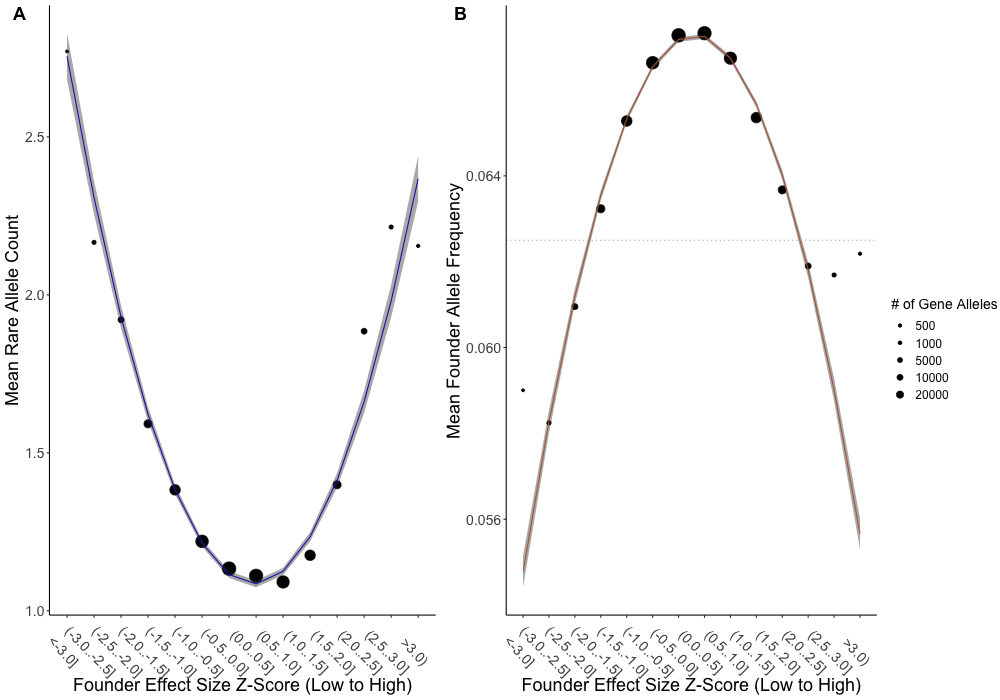
\includegraphics[width=0.8\textwidth,height=3in]{figures/chapter2_figure4.png}
%\protect\rule{0ex}{5ex}
\caption{\textbf{Dysregulation and Stabilizing Selection on local-eQTL} \textbf{A} Abundance of rare alleles is associated with extreme expression.
The x-axis shows the Z-score of founder effect sizes broken into bins.
The y-axis shows the average number of rare alleles located within 5kb upstream of genes.
Points represent gene founder alleles with effect size Z-scores within a range, with the size of the points relative to the number of gene alleles within the bin.
The blue line is a quadratic model weighted by the number of gene alleles per bin.
\textbf{B} Extreme founder alleles are at lower frequency.
The y-axis shows the founder allele frequency in the BALANCE population.
The grey dashed line is the expected balanced frequency if all founders were equally represented (0.0625).
The red line is a quadratic model weighted by the number of gene alleles per bin.}
\label{fig:smile_frownfigure}
\end{figure*}
Interestingly, none of the "usual suspects" for these two QTL appear as candidate genes, or even have strong correlations of effect sizes compared to other overlapping eQTL (Figures \ref{fig:chapter2_supfigure4} \& \ref{fig:chapter2_supfigure5}).
\textit{qDTA8} is in the same location on chromosome 8 as two well-characterized flowering time QTL, \textit{vgt1} and \textit{vgt2}.
The causal genes for these two QTL are \textit{ZmRap2.7} (Zm00001d010987) and \textit{ZCN8} (Zm00001d010752), respectively.
Previous research regarding the causal variants impacting the expression of these genes would lead us to expect that they would show up as local-eQTL \citep{Guo,Castelletti}.
\textit{ZmRap2.7} was expressed at a detectable level in only one timepoint, T20.
The gene did have a local-eQTL, and its effect size was moderately negatively correlated with the effect sizes of \textit{qDTA8} in St. Paul, 2017 \#1 (r = -0.45, Figure \ref{fig:chapter2_supfigure4}).
The negative correlation is consistent with our understanding of \textit{ZmRap2.7}'s impact on flowering, but the magnitude of the correlation is markedly lower than the $\max {|r_{local}|}$ for \textit{qDTA8}.
\textit{ZCN8} was expressed in all timepoints and had significant local-eQTL in all but one timepoint, T18.
The local-eQTL effect sizes were weakly correlated with \textit{qDTA8} effect sizes in any timepoint.
\textit{ZmMADS69} was identified as the causal gene for \textit{vgt3}, a previously identified flowering time QTL on chromosome 3 that is in the same location as \textit{qDTA3-2} \citep{Liang}.
The eQTL effect sizes for local-eQTL for \textit{ZmMADS69}, which were found in all four timepoints, were moderately correlated with qDTA3-2 effect sizes in St. Paul, 2017 \#1, ranging from r = 0.43 in T12 to r = -0.50 in T20 (Figure \ref{fig:chapter2_supfigure5}).
Similarly, the magnitude of these correlation is markedly lower than the $\max {|r_{local}|}$ for \textit{qDTA3-2}.
The reversal in the direction of correlation for \textit{ZmMADS69} is also interesting to note.
Overall, we find that the founder effect sizes of local-eQTL for known flowering time QTL candidate genes ranged from weakly to moderately correlated with QTL effect sizes, and were all less correlated with their respective QTL than the $\max {|r_{local}|}$.
\par
One drawback of this method of identifying candidate genes is that it does not account for distal-eQTL that are truly associated with QTL.
There were a number of QTL where there high correlations between local-eQTL and distal-eQTL, such that they did not pass our signficance threshold, but are still of note.
Two QTL had $\delta_z < 0$ where the distal-eQTL was more strongly correlated with the QTL than the local-eQTL than expected by chance. 
For a QTL for TKW found in Graneros, 2015 \textit{qTKW7-2}, the most correlated local-eQTL was for Zm00001d020593 in T12 (r = 0.72) and the most correlated distal-eQTL was for Zm00001d052810 in T12 (r = 0.96).
For another QTL from Graneros, 2015 for HGM, \textit{qHGM7}, which overlaps with \textit{qTKW7-2}, the most correlated local-eQTL was for  Zm00001d020687 in T12 (r = -0.777) and the most correlated distal-eQTL was for Zm00001d047181 in T12 (r = 0.941).
Two other QTL did not differ significantly from permutations in their $\delta_z$ values, but had higher local-eQTL correlations than most QTL.
In St. Paul, 2017 \#1, a TKW QTL, \textit{qTKW2}, had a local-eQTL for Zm00001d002677 in T12 (r=-0.958) and a distal-eQTL for Zm00001d034373 in T12 (r= 0.962).
Lastly, a QTL for TPH BLUPs, \textit{qTPH1}, had a local-eQTL for Zm00001d027904 in T12 (r=0.894) and a distal-eQTL for Zm00001d049254 in T12 (r = -0.892).
\subsection{eQTL Associated With Complex Traits Tend to have Small Effect Sizes}
One explanation for the disparity in the ability eQTL to explain QTL for complex traits is that eQTL mapping is poorly powered to detect eQTL associated with complex traits due to the impacts of selection \citep{Mostafavi}.
Consistent with this explanation, we find a significant negative relationship between the significance ranking of local-eQTL that overlap QTL SIs and the correlation with QTL founder effect sizes (F-value = 13.11, p-value = 2.94e-4).
In addition, the local-eQTL for all 5 candidate genes were of relatively small effect size compared to the largest effect eQTL in the QTL support interval (\hyperref[fig:candidates]{Figure 3}B).
The -log10(p-values) of the 5 candidate genes range from 1.12 to 0.16, meaning they would most likely not pass more stringent significance thresholds.
This is in the lower 13\% of -log10(p-values) for identified local-eQTL.
The proportion of variation in expression explained by the 5 candidate genes ranged from 15-20\%.
There was no significant relationship between the proportion of phenotypic variation explained by a QTL and the $\max_{|r_{local}|}$ eQTL for the QTL (Figure \ref{fig:chapter2_supfigure6}).
Overall, these results are inline with the idea that eQTL that mediate complex traits will tend to have smaller effect sizes, and will not be detected by most eQTL studies.

\subsection{Rare Allele Burden and Dysregulation of Expression}
Stabilizing selection will reduce the frequency of large-effect alleles in a population over generations.
For this reason, deleterious alleles tend to be rare.
Alleles that are outside of coding regions, although not impacting the function of a protein, can still be deleterious if they disrupt or alter the expression of genes.
\cite{Zhao} identified a relationship between the number of rare alleles within the regulatory region of a gene and strong deviations from average gene expression.
This pattern was also observed in a maize association panel looking at deviations of total gene expression from the population average \citep{Kremling2}.
We looked for the same relationship using mean-standardized founder effect sizes from local-eQTL, where we can look at the local genetic effect on expression, rather than total expression.
Using around 2 million variants that are rare in maize (0.01 $\ge$ MAF $\ge$ 0.05) but segregating in the BALANCE founders, we found a significant relationship between extreme founder effect sizes on expression and the number of rare alleles within a 5kb window upstream of those genes (\hyperref[fig:smile_frownfigure]{Figure 4}A).
Founder alleles with more extreme expression tended to possess more rare alleles on average than founder loci with intermediate expression, fitting a quadratic model (p-value = 2.2e-06, t-value = 8.611).
This pattern was also observed using ranks of founder effect sizes (p-value = 1.10e-8, t-value = 12.65, Figure \ref{fig:chapter2_supfigure7}).
This relationship is consistent with historical stabilizing selection bringing alleles associated with extreme expression to lower frequency in maize.
In addition to historical stabilizing selection, this population allowed us to test for evidence of stabilizing selection that occurred over the course of making the BALANCE population.
Previously, it had been shown that many regions displayed evidence of segregation distortion in the BALANCE population, with significant over- or under-representation of certain founder alleles \citep{Odell}.
We tested to see if there was a relationship between the extreme expression associated with a founder allele and its frequency in the population.
Across local-eQTL for the 5000 most highly expressed genes, extreme founder effect sizes tended to be at lower allele frequencies (\hyperref[fig:smile_frownfigure]{Figure 4}B).
This relationship was fit to a negative quadratic model (p-value=9.9e-9,t-value=15.20) and is consistent with a pattern of recent stabilizing selection reducing the frequency of large effect founder alleles in the population.

%\begin{SCfigure*}
\begin{figure}[!ht]
\centering
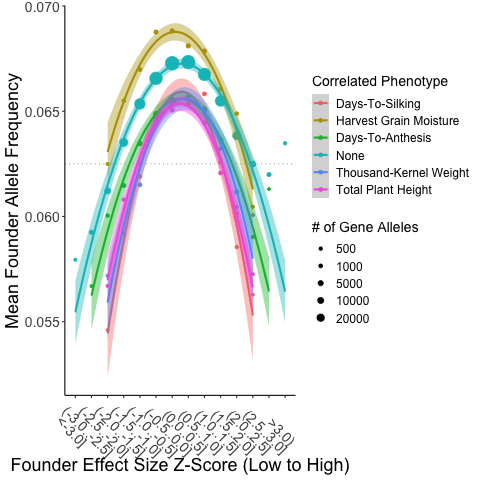
\includegraphics[width=0.5\textwidth,height=3in]{figures/frown_quad.png}
%\protect\rule{0ex}{3ex}
\caption{\textbf{Selection on Genes Expression Associated with Complex Traits}
The x-axis shows the Z-score of founder effect sizes broken into bins.
The different colors show the least square means estimated from a quadratic model broken up by the complex trait a gene was associated with.
The y-axis shows the founder allele frequency.
The grey dashed line is the expected balanced frequency if all founders were equally represented (0.0625).}
\label{fig:pheno_frownfigure}
\end{figure}
%\end{SCfigure*}

\subsection{Selection on Genes Associated with Complex Traits}
The breeding scheme of the population intentionally kept extreme alleles associated with flowering time segregating at appreciable frequencies to increase the chance of finding flowering time QTL.
In the initial F1s, early and late flowering founders were intentionally crossed to one another.
Further, in the three generations of intercrossing of synthetic lines, there was an abundance of crosses made between lines with similar flowering times.
As a result, there was intentional diversifying selection on flowering time applied to this population.
We previously found genomic evidence of selection on flowering time, with flowering time genes enriched in regions of high inter-chromosomal LD in the  BALANCE population \citep{Odell}.
We, therefore, wished to look for evidence of selection on gene expression associated with complex traits, with a particular focus on flowering time.
To do this, we split local-eQTL by if they overlapped with a QTL SI and had founder effect sizes that correlated with those QTL.
Across all groups, the relationship between founder effect size Z-score and founder allele frequency was still consistent with stabilizing selection (F-value=4256.49, p-value $<$ 2.2e-16), although there was a significant effect of association with complex traits (F-value=182.65, p-value $<$ 2.2e-16, \hyperref[fig:pheno_frownfigure]{Figure 5}).
Although there was a significant interaction between group and the second degree polynomial of the quadratic model, there was not a significant second degree polynomials among groups in a pairwise comparison.
Although we were unable to detect a significant difference in the steepness of the quadratic for the eQTL associated with complex traits, three traits, DTS, TKW, and TPH, appeared to have more narrow parabolas than HGM, DTA, and None, suggesting stronger stabilizing selection acting on expression of genes associated with those traits more than the others.
HGM and DTA, displayed slightly wider parabolas than the other traits.
For HGM, it may be that this trait is less directly related to fitness.
For eQTL associated with DTA, this pattern is consistent with diversifying selection, which would increase the frequency of large-effect loci.

%%%%%%%%%%%%%%%%%%%%%%%%%%%%%%%%%%%%%%%%%%%%%%%%%%%%%%
\section{Discussion}
%%%%%%%%%%%%%%%%%%%%%%%%%%%%%%%%%%%%%%%%%%%%%%%%%%%%%%

\subsection{Biological Insights from Integrative QTL-eQTL Analysis}
We combined eQTL mapping and QTL mapping in a MAGIC population and identified five candidate genes associated with two flowering time QTL (Table \ref{tab:candtable}).
The three candidate genes we identify for \textit{qDTA3\_2} have not previously been associated with flowering time.
The gene Zm00001d042291 encodes Zinc finger homeobox protein 4 that functions in RNA polymerase II complex binding and mRNA processing
It has previously been found to be associated with node length and leaf angle \citep{Wallace} and overlaps with a GWAS hit for ear height \citep{Peiffer2}. 
Zm00001d041900 is a hypothetical protein with a Nrap protein domains, and it has predicted involvement in RNA binding, rRNA processing, and tRNA export from nucleus.
It was found to be associated with leaf chlorophyll A and B content \citep{Wallace} and also overlaps with a GWAS hit for ear height \citep{Peiffer2}.
Zm00001d042306 (\textit{shrek1}– shrunken and embryo defective kernel1) encodes an anaphase-promoting complex subunit 4-like WD40 domain-containing protein.
This gene is known to play a crucial role in kernel development and ribosome biogenesis.
Most of the research into this gene has been surrounding kernel development, due to the fact that \textit{shrek1} mutants are embryo-lethal \citep{Liu8}. 
However, there is some previous association with reproductive development and flowering.
Its ortholog in \textit{Arabidopsis} is \textit{COP1}, which is involved in light-regulated growth, and has been found to play a role in flowering through interaction with a number of known flowering time regulators \citep{Jang,Yu4,Yang2}.
In maize, it has been associated with tassel branch number and  node number \citep{Wallace}.
It also overlaps with a GWAS hit for plant height \citep{Peiffer2} and is 5kb downstream of a GWAS hit for hundred-kernel weight \citep{Zhang5}.

The two candidate genes we identify for \textit{qDTA8}, similarly, are not strongly linked to flowering from previous understanding.
Zm00001d011123 is a RanBP2-type domain containing Zinc finger protein.
It was found to be a candidate gene for source-sink-regulated senescence in maize \citep{Kumar} and overlaps a QTL hit for maize streak virus reaction \citep{Nair}.
Zm00001d011294 is a Rho GTPase-activating protein (RhoGAP) whose ortholog in \textit{Arabidopsis}, \textit{REN1}, is involved in cell tip expansion and pollen tube development \citep{Hwang}.
The gene is around 17kb downstream of a QTL for coefficient of variation of days to anthesis \citep{Li4}
\par
There are a few interesting observations on the nature of the candidate genes identified.
For one, with our method of determining candidate genes, 4 of the 5 significant candidates were identified from expression and phenotype effect sizes in the same year and location in two separate fields (St. Paul, 2017 \#1 \& \#2).
The last candidate gene was correlated with phenotype effect sizes from Blois, 2017, which is located 203 km from St. Paul, France; of the environment-years from which phenotypes were sampled, this is the geographically and temporally closest to St. Paul.
In addition, the candidate genes, although all identified from local-eQTL in the first timepoint, T12, were all distinct, despite several of them being correlated with presumably the same QTL in different environment-years.
One explanation for the fact that we only find strong candidate genes in T12 is that this was the most relevant timepoint for flowering, given that the plants had begun to initiate flowering at T12 and were experiencing more extreme stress in later timepoints.
These finding provide some support for the hypothesis that eQTL fail to explain as much of GWAS hits as we would expect due to the fact that gene expression is not being measured in the appropriate contexts, whether that be time, tissue, developmental stage, or external stimulus.
\subsection{The Ability of eQTL to Explain Complex Traits}
The use of integrative methods to identify candidate genes that mediate complex traits has been ongoing.
The multi-allelic nature of the BALANCE population offers a unique opportunity to directly assess if the genetic effects of a locus on gene expression and complex traits are correlated.
The correlation of QTL and eQTL founder effect sizes provides evidence for the role of a genetic variant in mediating a QTL, ruling out overlap simply due to linkage (Figure \ref{fig:scenarios}).
However, our method cannot reject that the correlation is due to pleiotropy, rather than mediation.
Notably, all of the 5 candidate genes that we identify have not previously been associated with flowering, but do overlap with some GWAS hits for growth-related traits.
It seems very possible that the correlation we see is more a reflection of pleiotropy than mediation.
In addition, the two QTL that have significantly correlated local-eQTL both have well-characterized causal genes that are not among our five candidate genes (\textit{ZmRap2.7} and \textit{ZCN8} for \textit{qDTA8} and \textit{ZmMADS69} for \textit{qDTA3\_2}).
This, again, highlights the importance of gene expression context in the usefulness of such studies.
It is very possible that even the earliest timepoint, T12, is too late in development to capture the effects on gene expression of these known causal genes.
\par
It is unclear what degree of correlation between founder effect sizes is biologically meaningful.
The method we apply to identify candidate genes is stringent, and may filter out many true positives.
In particular, in using correlations from distal-eQTL overlapping QTL as our null expectation, we ignore that some of these distal-eQTL may be truly biologically associated with the QTL.
Both local-eQTL and distal-eQTL may be either \textit{cis}- or \textit{trans}-acting and there is evidence of long-range \textit{cis}-regulatory elements in maize, which might show up as distal-eQTL on the same chromosome in our study and would not be considered in our search for candidate genes \citep{Ricci}.
Due to this, we may miss a number of true positives applying this method of determining significance.
\par
Although we only considered the gene with the highest local-eQTL correlation as a candidate gene, within QTL SIs there were a number of genes with relatively high correlations with QTL effect sizes.
This is consistent with the concept of expression piggybacking, where multiple neighboring genes share correlated effects of local-eQTL, presumably due to shared chromatin modification \citep{Ghanbarian,Wang3}.
This complicates the identification of candidate genes, as multiple genes in a genomic region may have similar local-eQTL effects.
However, in maize, many of these consecutive correlated gene clusters shared similar functions, suggesting that genes that share local-eQTL effects tend to be involved in the same regulatory networks \citep{Wang3}.
\subsection{Impact of Stabilizing Selection on Expression}
Stabilizing selection brings alleles with extreme effect sizes to lower frequency.
Therefore, we might expect eQTL that are strongly correlated with complex traits to be select against.
Similarly, eQTL with the largest effect sizes would likely not be strongly associated with complex traits \citep{Mostafavi}.
We find a negative relationship between local-eQTL significance and correlation with QTL for complex traits.
Similarly, the local-eQTL for the 5 candidate genes all had small effect sizes relative to the most significant eQTL that overlapped their QTL support intervals (Figure \ref{fig:candidates}B).
These findings are consistent with selection against genetic variants with large effects on complex traits.
Negative selection on alleles with large effects on complex traits will disproportionately impact the power of eQTL mapping over QTL mapping or GWAS.
This is due to the fact that the power to detect an eQTL is dependent on a genetic variant's impact on expression, while the power to detect an eQTL is dependent on a genetic variant's impact on a complex trait.
For eQTL, we have shown that there is evidence of both historical and recent stabilizing selection bringing alleles with extreme effects on expression to low frequency.
This could result in eQTL that have a large effect on gene expression and on a complex trait either not passing significance, or being among the lower rankings of significance.
Even in a species such as maize, where selection from domestication has had a large influence on many traits, we still find that stabilizing selection has strongly shaped the genetic architecture of gene expression traits.
For natural populations, we might expect this effect to be even stronger.
\par
We find a strong relationship between the number of rare alleles within gene regulatory regions and extreme expression (Figure \ref{fig:smile_frownfigure}A). 
We also show that founder alleles associated with extreme expression tended to be at lower frequency in the population, consistent with extreme expression being deleterious (Figure \ref{fig:smile_frownfigure}B).
These results provide compelling evidence of both historical and recent stabilizing selection.

\section{Conclusion}
We utilize estimates of founder effect sizes for QTL and eQTL to identify candidate genes, and examine the impacts of selection on gene expression traits.
We provide evidence that the success of integrative QTL-eQTL studies may be mitigated both by the appropriateness of the expression data to the complex trait and by the impact of stabilizing selection on the power of eQTL studies.
Finally, we provide further support for the role of rare alleles in the dysregulation of gene expression.
Overall, we highlight collecting gene expression data from relevant contexts to the phenotype being measured as playing a crucial role in the efficacy of eQTL studies to explain QTL.
Combined, our findings reinforce stabilizing selection as a strong influence on the genetic architecture of gene expression, generally.
For genes associated with complex traits, generally, we see that more extreme alleles are even more heavily penalized.
However, diversifying selection on days-to-anthesis may have increased the frequency of alleles associated with extreme expression of genes associated with male flowering.

\section{Acknowledgments}
We would like to acknowledge the Limagrain breeding support and trialing team for producing the doubled haploids and running the field trials, and collecting the tissue for the expression data used in this study, as well as our funding sources, the University of California, Davis Department of Plant Sciences and NSF grant 1754098.

\bibliography{balance_rna}

\beginsupplement
\onecolumn
\section*{Supplement}

\begin{figure}[!ht]
\centering
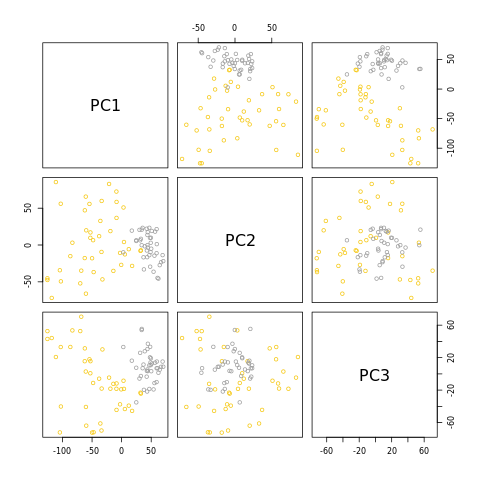
\includegraphics[width=0.5\textwidth,height=3.5in]{figures/exp_WD_0712_PC_pairs.png}
\caption{\textbf{First Three Principal Components of Normalized Gene Expression in T12}. Color indicates the plate of the sample.}
\label{fig:chapter2_t12pc}
\end{figure}

\begin{figure}[!ht]
\centering
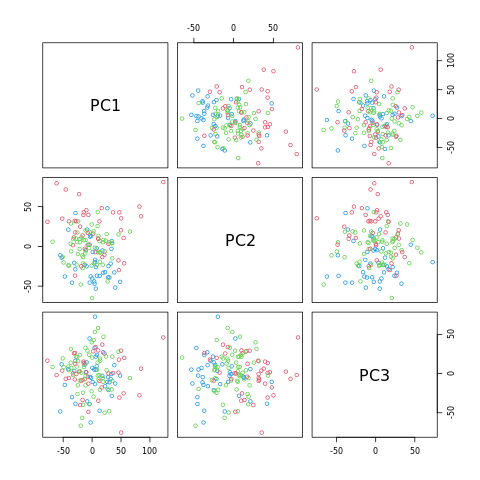
\includegraphics[width=0.5\textwidth,height=3.5in]{figures/exp_WD_0718_PC_pairs.png}
\caption{\textbf{First Three Principal Components of Normalized Gene Expression in T18}. Color indicates the plate of the sample.}
\label{fig:chapter2_t18pc}
\end{figure}

\begin{figure}[!ht]
\centering
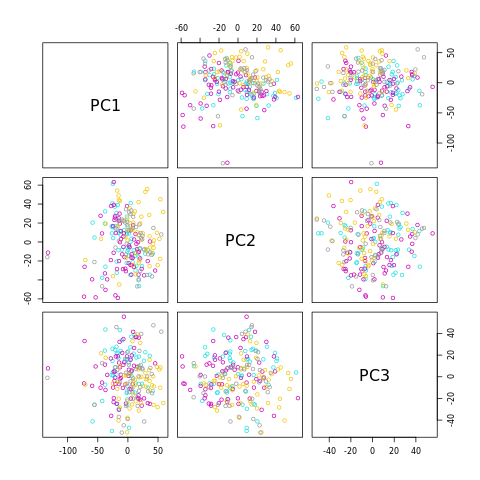
\includegraphics[width=0.5\textwidth,height=3.5in]{figures/exp_WD_0720_PC_pairs.png}
\caption{\textbf{First Three Principal Components of Normalized Gene Expression in T20}. Color indicates the plate of the sample.}
\label{fig:chapter2_t20pc}
\end{figure}

\begin{figure}[!ht]
\centering
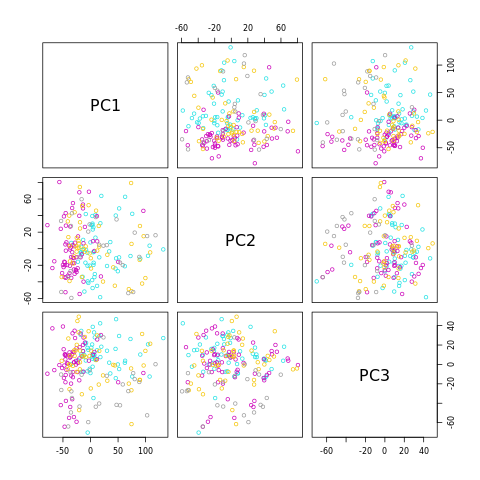
\includegraphics[width=0.5\textwidth,height=3.5in]{figures/exp_WD_0727_PC_pairs.png}
\caption{\textbf{First Three Principal Components of Normalized Gene Expression in T27}. Color indicates the plate of the sample.}
\label{fig:chapter2_t27pc}
\end{figure}

\begin{figure}[!ht]
\centering
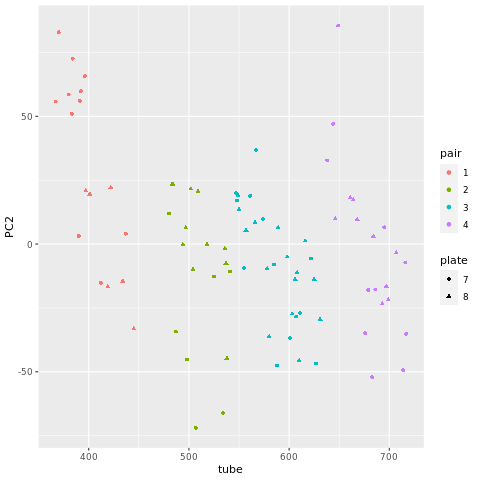
\includegraphics[width=0.7\textwidth,height=3.5in]{figures/WD_0712_PC2_pair_tube.png}
\caption{\textbf{PC2 of Normalized Gene Expression in T12}. The x-axis is the tube number of a sample, which is representative of the order of sampling within sampling group. The color represents the sampling group, or pair of samplers. The shape represents the plate of the sample.}
\label{fig:chapter2_t12pc2}
\end{figure}

\begin{figure}[!ht]
\centering
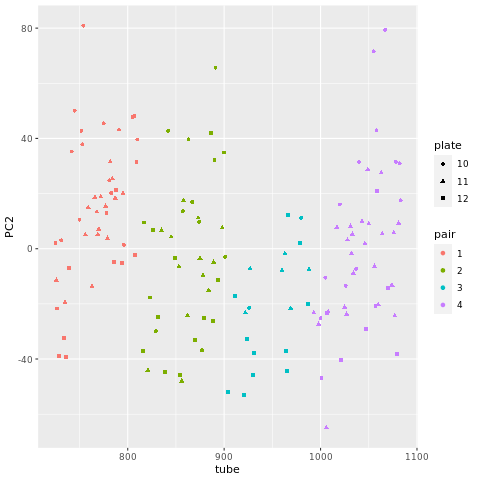
\includegraphics[width=0.7\textwidth,height=3.5in]{figures/WD_0718_PC2_pair_tube.png}
\caption{\textbf{PC2 of Normalized Gene Expression in T18}. The x-axis is the tube number of a sample, which is representative of the order of sampling within sampling group. The color represents the sampling group, or pair of samplers. The shape represents the plate of the sample.}
\label{fig:chapter2_t18pc2}
\end{figure}

\begin{figure}[!ht]
\centering
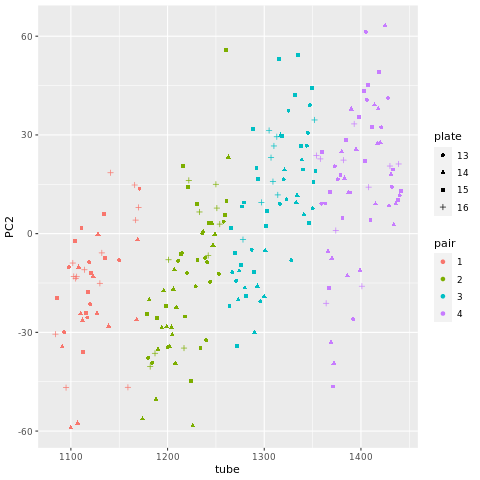
\includegraphics[width=0.7\textwidth,height=3in]{figures/WD_0720_PC2_pair_tube.png}
\caption{\textbf{PC2 of Normalized Gene Expression in T20}. The x-axis is the tube number of a sample, which is representative of the order of sampling within sampling group. The color represents the sampling group, or pair of samplers. The shape represents the plate of the sample.}
\label{fig:chapter2_t20pc2}
\end{figure}

\begin{figure}[!ht]
\centering
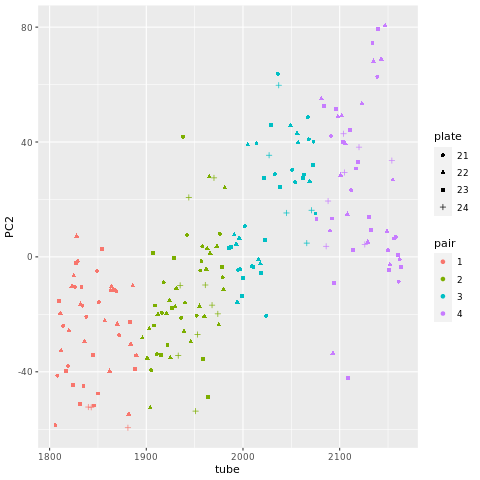
\includegraphics[width=0.7\textwidth,height=3in]{figures/WD_0727_PC2_pair_tube.png}
\caption{\textbf{PC2 of Normalized Gene Expression in T27}. The x-axis is the tube number of a sample, which is representative of the order of sampling within sampling group. The color represents the sampling group, or pair of samplers. The shape represents the plate of the sample.}
\label{fig:chapter2_t27pc2}
\end{figure}

\begin{figure}[!ht]
\centering
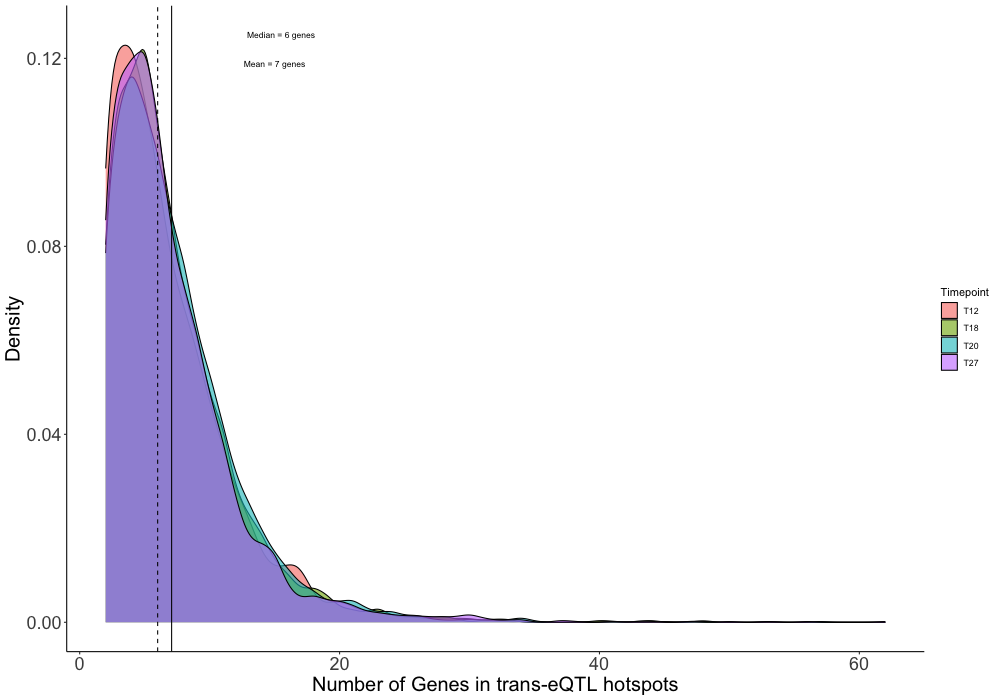
\includegraphics[width=0.7\textwidth,height=3in]{figures/trans_eQTL_hotpsots.png}
\caption{\textbf{Density Distribution of Genes Affected by distal-eQTL Hotspots}. We consider markers that were distal-eQTL for more than one gene within a timepoint as distal-eQTL, with color representing timpeoint}
\label{fig:chapter2_supfigure1}
\end{figure}

\begin{figure}[!ht]
\centering
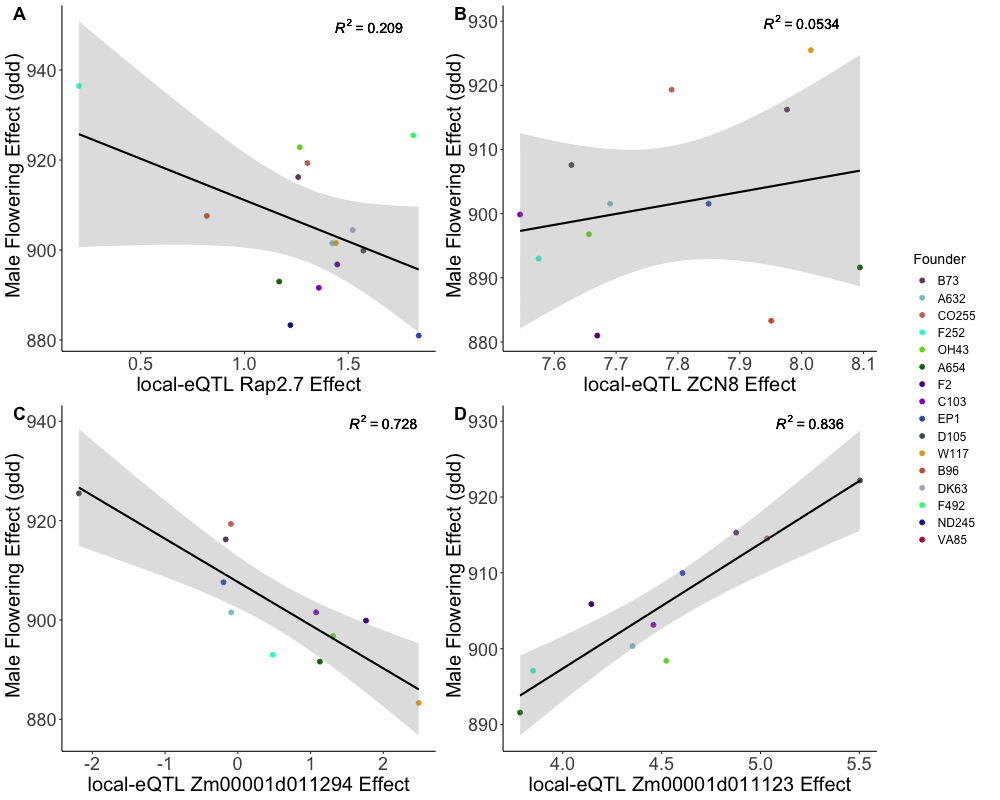
\includegraphics[width=0.9\textwidth,height=3.5in]{figures/chapter2_figure5.png}
\caption{\textbf{Correlation of Founder Effect Sizes for Candidate Genes and Known FT genes for \textit{qDTA8}}. \textbf{(A)} \textit{ZmRap2.7}, the gene impacted by \textit{vgt1}. 
\textbf{(B)} \textit{ZCN8}, the causal gene for \textit{vgt2},
\textbf{(C)} Zm00001d011294, and \textbf{(D)} Zm00001d011123.}
\label{fig:chapter2_supfigure4}
\end{figure}


\begin{figure}[!ht]
\centering
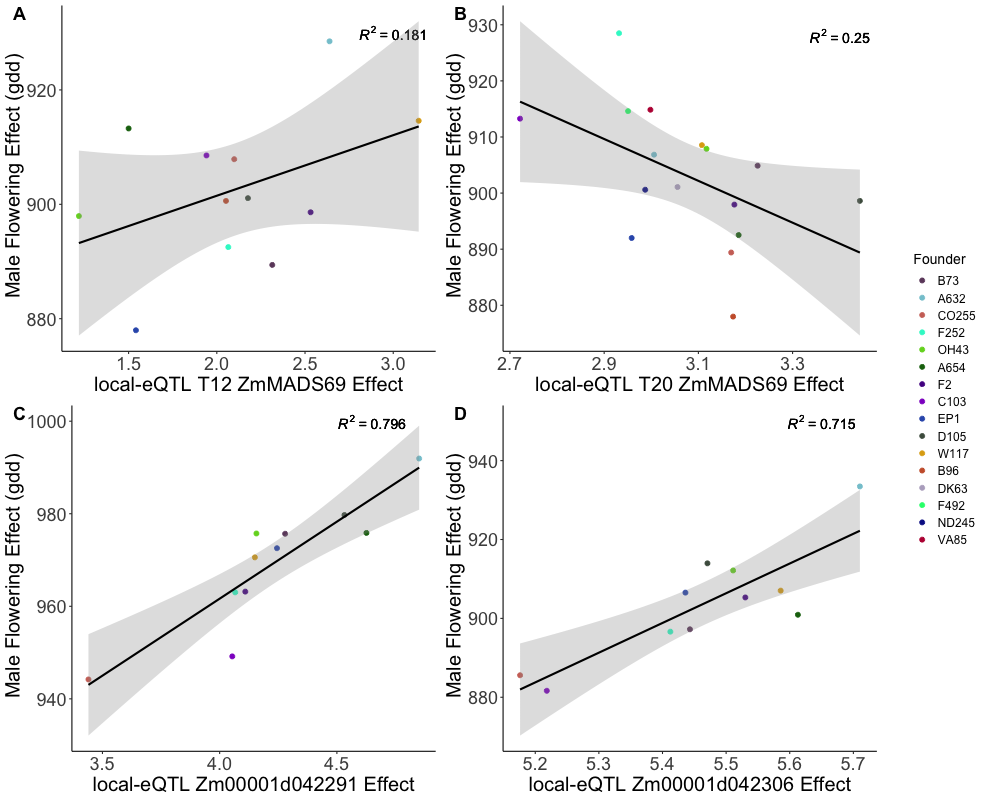
\includegraphics[width=0.9\textwidth,height=3.5in]{figures/chapter2_figure6.png}
\caption{\textbf{Correlation of Founder Effect Sizes for Candidate Genes and Known FT genes for \textit{qDTA3-2}}. \textit{ZmMADS69}, the causal genes for \textit{qDTA3-2} in timepoint \textbf{(A)} T12  and \textbf{(B)} T20,
\textbf{(C)} Zm00001d042291, and \textbf{(D)} Zm00001d042306.}
\label{fig:chapter2_supfigure5}
\end{figure}

\begin{figure}[!ht]
\centering
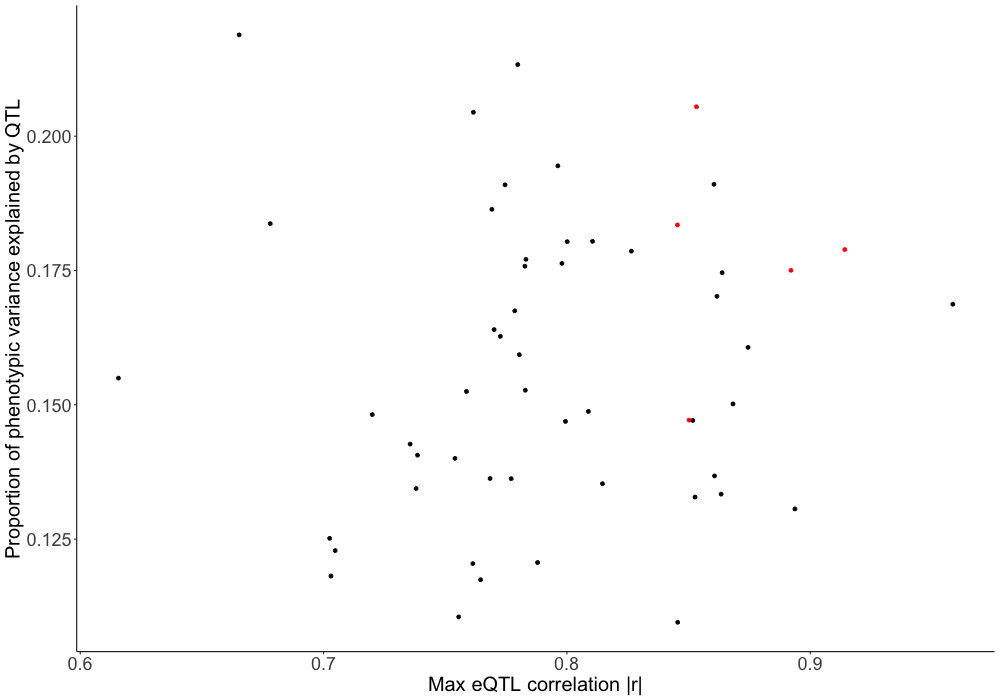
\includegraphics[width=0.7\textwidth,height=3in]{figures/eQTL_r_by_QTL_propvar.png}
\caption{\textbf{Relationship between Max local-eQTL $|r|$ and Proportion of Phenotypic Variation Explained by QTL}}
\label{fig:chapter2_supfigure6}
\end{figure}

\begin{figure}[!ht]
\centering
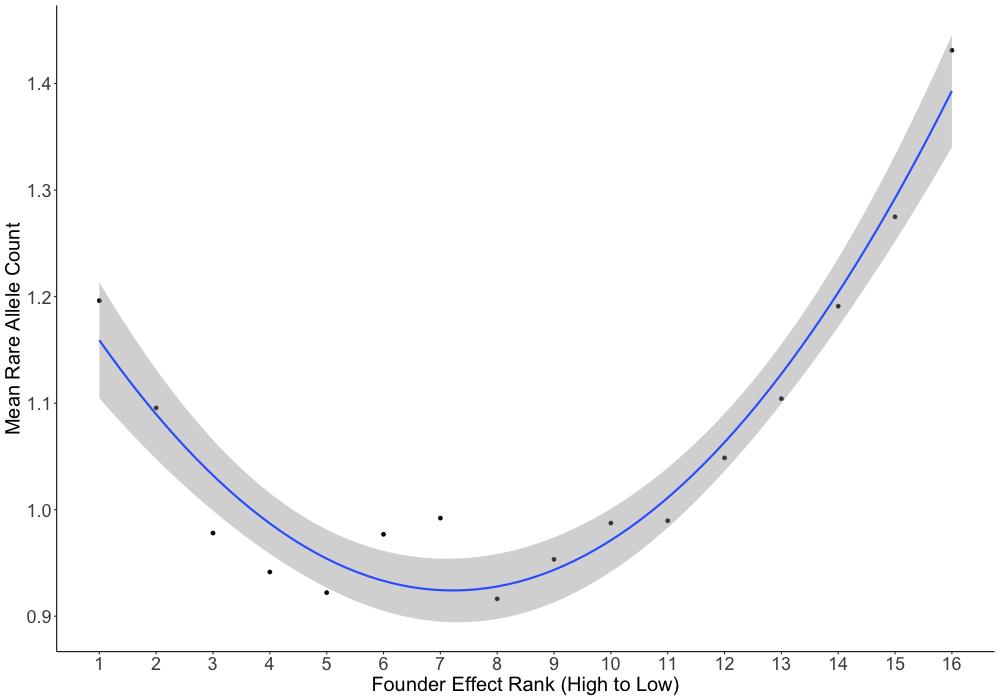
\includegraphics[width=0.7\textwidth,height=3in]{figures/smile_beta_rank_plot.png}
\caption{\textbf{Relationship Between Average Rare Allele Count and Rank of Founder Effect Size}}
\label{fig:chapter2_supfigure7}
\end{figure}

\begin{table*}
%\renewcommand{\familydefault}{\sfdefault}\normalfont
\centering
\caption{\bf Information on BALANCE Founder Lines and Tester}
\label{tab:founder_suptable}
\begin{adjustbox}{max width=0.98\textwidth,center}
\begin{tabular}{c c c c c c}
\hline \hline \\
Name & Status & Year of Release & Pedigree & Group & Sub-group \\
\hline \\
A632 & Founder & 1964 & (Mt42$\times$ B14) $\times$ B14)$^3$ & Dent & BSSS \\
A654 & Founder & 1969 & A116 $\times$ Wf9 & Dent & Miscellaneous \\
B73 & Founder & 1974 & BSSS C5 & Dent & BSSS \\
B96 & Founder & 1958 & Maize Amargo from Argentina & Flint & - \\
C103 & Founer & 1974 & Lancaster Sure Crop & Dent & Lancaster \\
CO255 & Founder & 1978 & (F7 $\times$ EP1) $\times$ (F115 $\times$ W33) & Miscellaneous (50\% Flint, 50\% Minnesota 13) & - \\
D(K)105 & Founder & 2003 & Gelber Badischer Landinario population & European Flint & - \\
D(K)63 & Founder & 1991 & Unknown (BSSS x Iodent) & Dent & Miscellaneous \\
EP1 & Founder & 1974 & Lizargarote population (Spain) & European Flint & - \\
F(V)2 & Founder & 1965 & Lacaune population (France) & European Flint & - \\
F(V)252 & Founder & 1980 & F186 $\times$ CO125 & Dent & Miscellaneous \\
F492 & Founder & 1980 & F556 $\times$ F575 & Dent & Miscellaneous \\
ND245 & Founder & 1979 & W755 $\times$ W7771 & Dent & - \\
OH43 & Founder & 1961 & V8 $\times$ OH40b & Dent & Lancaster \\
VA85 & Founder & 1977 & Virginia Long Ear Synthetic population & Dent & M14:Oh43 \\
W117 & Founder & 1968 & W643 $\times$ Minnesota 13 & Dent & M13 \\
MBS847 & Tester & 1983 & Developed from a commercial variety & Dent & Iodent \\
\hline
\end{tabular}
\end{adjustbox}
\end{table*}
\endsupplement
\end{document}
